\section{Estrellas de neutrones}\label{sc:intro}

Las estrellas de neutrones aparecen en el universo como el remanente de la muerte de una estrella masiva (pero no tan masiva como para convertirse en un agujero negro).
Cuando nace una estrella consume principalmente Hidrógeno, produciendo Helio en el proceso.
Unos $10^{10}$ años después el Hidrógeno se agota y la estrella, que ya no puede compensar la compresión gravitatoria, se contrae y se calienta.
Esto le permite comenzar a fusionar Helio, que vuelve a generar suficiente presión para evitar el colapso gravitatorio.
A medida que envejece, una estrella va consumiendo y agotando sucesivamente hidrógeno, helio, carbono, neón, oxígeno y silicio.
Cada vez que la estrella agota un tipo de combustible se produce el proceso mencionado: el núcleo se contrae, se calienta y comienza a consumir un nuevo combustible que, generalmente, es el producto de la fusión del anterior.
Esto se conoce como la ``secuencia principal'' de una estrella~\cite{woosley_physics_2005}.
Para poder fusionar elementos cada vez más pesados, una estrella requiere mayor temperatura, y sólo estrellas muy masivas (con masa mayor a 8 veces la masa solar) pueden completar la secuencia.
El producto de la fusión de silicio (la última etapa de la secuencia) es principalmente hierro y, dada su alta energía de unión, no es posible extraerle energía por fusión.
En la etapa del silicio (que dura apenas un par de semanas), casi toda la presión que evita el colapso es provista por un gas degenerado de electrones.
Cuando la masa del núcleo alcanza el límite de Chandrasekhar de aproximadamente $1.4\,M_\odot$, los electrones se vuelven ultra-relativistas (modificando así su ecuación de estado) y no pueden seguir soportando el núcleo a través de la presión de degeneración.
En esta etapa, el núcleo de la estrella es muy inestable.
Existen dos procesos que absorben energía (conocidos como refrigerantes estelares): la fotodesintegración de los núcleos y la captura de electrones.
En la fotodesintegración, la energía cinética es usada para separar núcleos atómicos y en la captura de electrones la energía cinética de los electrones se transforma en energía cinética de neutrinos que escapan de la estrella.
Estos procesos son tan efectivos que el colapso del núcleo estelar es prácticamente inevitable.

A esas densidades, los electrones comienzan a ser capturados por los núcleos de hierro, aumentando la proporción de neutrones y privando al núcleo estelar de la presión ejercida por el gas de electrones.
Esto precipita el colapso gravitatorio del núcleo, que comienza a comprimirse violentamente a una velocidad de $0.25c$.
A medida que la compresión avanza y la densidad aumenta y llega a niveles de la densidad nuclear, comienzan a tomar relevancia la degeneración de neutrones y las fuerzas nucleares.
Éstas resisten la compresión y detienen el colapso cuando el núcleo se vuelve dos o tres veces más denso que la materia nuclear normal.
El núcleo luego rebota fuertemente y comienza una onda de choque que viaja a través del material que viajaba originalmente hacia el centro.
Esta onda de choque puede revertir la caída de la materia de estrellas que envuelve al núcleo y producir una expulsión hacia afuera, llamada supernova.

La física del colapso, el rebote y la onda de choque asociada es muy complicada.
No es seguro cómo se transfiera la energía y el momento a las capas exteriores de la estrella, y tampoco es seguro que el colapso del núcleo esté siempre acompañado por una supernova.
De todos modos, el colapso deja un residuo del núcleo: una proto-estrella de neutrones caliente (con temperaturas de entre $20$ y $50\,\text{MeV}$).
Esa proto-estrella de neutrones va acreciendo material de las capas exteriores de la estrella y, si no se convierte en un agujero negro, se enfría hasta estabilizarse (principalmente a través de la emisión de neutrinos) formando un núcleo rico en neutrones de aproximadamente $10\,\text{km}$ de radio: una estrella de neutrones propiamente dicha.
Durante esta etapa, la proto-estrella de neutrones emite hasta un 10\% de su masa en reposo en forma de neutrinos, y se cree que la interacción de estos neutrinos con el material de las capas exteriores de la estrella produce la Súper Nova, a pesar de que no hay consenso sobre los detalles del mecanismo~\cite{woosley_physics_2005, bethe_supernova_1990}.
También está en discusión el proceso de Urca como mecanismo de enfriamiento~\cite{piekarewicz_proton_2012, lattimer_direct_1991}, puesto que para algunos modelos de ecuación de estado la fracción de protones en equilibrio no sería suficiente como para producir la cantidad de neutrinos necesaria.
Durante este colapso, una gran parte de los electrones y los protones se transforman en neutrones a través de la captura de electrones, emitiendo neutrinos.
Debido a esto, la masa residual tiende a tener un exceso de neutrones por sobre protones, de ahí el nombre estrellas de neutrones.
Estas estrellas de neutrones entonces contienen protones y neutrones, pero además son eléctricamente neutros debido a los electrones: la carga neta es cero.

La masa de una estrella de neutrones es de entre 1 y 3 masas solares y su radio de cerca de $10\,\text{km}$, lo que resulta en una densidad de $\rho \simeq 10^{15}\,\text{g/cm}^3$, aproximadamente 20 veces mayor que la de los nucleos usuales.
Su estructura puede dividirse en dos partes, de acuerdo a modelos actuales~\cite{page_minimal_2004, geppert_temperature_2004}: la \emph{corteza}, de aproximadamente $1.5\,\text{km}$ de espesor y con una densidad de hasta la mitad de la densidad normal nuclear $\rho_0$; y el \emph{núcleo}, donde la estructura es aún desconocida y se mantiene altamente especulativa~\cite{akmal_equation_1998, ravenhall_structure_1983, oyamatsu_nuclear_1993, woosley_physics_2005}.

La densidad de dicha corteza toma los valores de la densidad nuclear normal ($\rho \simeq 10^{14}\,\text{g/cm}^3$ o $ \rho \simeq \rho_0=0.15 \text{fm}^{-3}$) a una profundidad $d \simeq 1\,\text{km}$, la densidad de \emph{neutron drip} ($\rho\simeq 4 \cdot 10^{11}\,\text{g/cm}^3$) a $d\simeq 0.5\,\text{km}$, y una mezcla de nucleos ricos en neutrones con densidades decrecientes hasta ser prácticamente cero en lo que se conoce como el envoltorio de la estrella de neutrones.
Ravenhall \emph{et al.} en Ref.~\cite{ravenhall_structure_1983} y Hashimoto \emph{et al.} en Ref.~\cite{hashimoto_shape_1984} propusieron que la corteza de las estrellas de neutrones está compuesta por estructuras conocidas como \emph{pasta nuclear}.

Varios modelos han sido desarrollados para estudiar la pasta nuclear, y han mostrado que estas estructuras aparecen debido al juego entre las fuerzas nuclears y las de Coulomb en un medio infinito.
De cualquier modo, la dependencia de los observables de diferentes cantidades termodinámicas no ha sido estudiado en profundidad.
Los trabajos originales de Ravenhall \emph{et al.}~\cite{ravenhall_structure_1983} y Hashimoto \emph{et al.}~\cite{hashimoto_shape_1984} utilizaban un modelo de gota líquida compresible, y mostraron que las \emph{fases de pasta}
--\emph{lasagna}, \emph{spaghetti} y \emph{gnocchi}-- son soluciones al estado fundamental de la materia de estrellas de neutrones.
De ahí en adelante, se han tomado distintos enfoques que clasificaremos en dos categorías: campo medio o microscópico.

Los trabajos de campo medio incluyen el modelo de la gota líquida, de Lattimer \emph{et al.}~\cite{page_minimal_2004}, Thomas-Fermi, de Williams y Koonin~\cite{williams_sub-saturation_1985}, entre otros~\cite{oyamatsu_nuclear_1993, lorenz_neutron_1993, cheng_properties_1997, watanabe_thermodynamic_2000, watanabe_electron_2003, nakazato_gyroid_2009}.
Los modelos microscópicos incluyen Dinámica Molecular Cuántica (QMD por sus siglas en inglés), usado por Maruyama \emph{et al.}~\cite{maruyama_quantum_1998, kido_md_2000} y por Watanabe~\emph{et al.}\cite{watanabe_structure_2003}, el Potencial Simple Semiclásico (SSP), utilizado por Horowitz~\emph{et al.}~\cite{horowitz_nonuniform_2004} y Dinámica Molecular Clásica (CMD), utilizado en nuestros trabajos previos~\cite{dorso_topological_2012}.
De todos los modelos utilizados para estudiar las estrellas de neutrones, las ventajas de los modelos clásicos o semiclásicos son la accesibilidad a las posiciones y velocidades de todas las partículas y el hecho de que no se debe especificar \emph{a priori} ninguna morfología específica, a diferencia de la mayoría de los modelos de campo medio.
Esto permite estudiar la estructura de la materia de estrellas de neutrones desde un punto de vista de las partículas.
En estos modelos la repulsión de Pauli entre nucleones del mismo isospín es, o bien considerado en la interacción nuclear, o bien agregado como un término aparte~\cite{dorso_classical_1988}.

La multifragmentación en sistemas nucleares fue estudiada
antes~\cite{bonasera_critical_2000, chikazumi_quantum_2001}, pero, a
diferencia de las colisiones, fue en mayor medida con materia nuclear (sin la interacción de Coulomb).
En un reciente trabajo de Caplan et al~\cite{caplan_pasta_2015}, se estudió la materia de estrellas de neutrones expandiéndose como posible explicación para la nucleosíntesis en colisiones de estrellas de neutrones y en otro trabajo, de este grupo~\cite{alcain_dynamics_2017}, la formación de los fragmentos en la expansión.

La compresión de la materia de estrellas de neutrones durante la colisión de dos estrellas es una posible fuente para nucleos a través del \emph{r-process}, como fue discutido inicialmente en Ref.~\cite{lattimer_black-hole-neutron-star_1974}.
De acuerdo a modelos hidrodinámicos~\cite{goriely_r-process_2011}, éstos tienen coeficientes de expansión típicos de  $\eta = 10^{-21}\,\text{c/fm} < \eta < 4\cdot 10^{-20}\,\text{c/fm}$.
Inspirados por la colisión de estrellas de neutrones, desarrollamos un estudio en la fragmentación de materia de estrellas de neutrones en expansión.

\section{Dinámica de los nucleones}\label{sc:nucleon}
Para estudiar la estructura nuclear de la corteza de las estrellas de neutrones es necesario comprender el comportamiento de los nucleones (es decir, protones y neutrones) a las densidades y temperaturas típicas de las capas externas de las estrellas.
Este conocimiento viene de décadas de estudio de la dinámica de nucleones a través del uso de modelos computacionales que han evolucionado, siendo cada vez más complejos.
En esta sección, revisamos esta evolución de los modelos, presentando una sinopsis de los modelos existentes y terminando con el modelo utilizado a lo largo de este trabajo: Dinámica Molecular Clásica (CMD).

\subsection{Evolución histórica de los modelos}
Varios enfoques se han utilizado para simular el comportamiento de la materia nuclear, especialmente en reacciones.
Los estudios iniciales, en mayor parte estadísticos, se desarrollaron hacia la década de 1980.
Éstos carecían de interacciones entre fragmentos y la dinámica de fragmentos luego de la colisión.
En la década del 1990 se agregaron estos efectos, resultando así en modelos más robustos~\cite{barz_cluster_1996}.
Todos estos modelos, sin embargo, estaban basados en geometrías idealizadas e ignoraban importantes fluctuaciones de forma y los efectos de la cinemática en la reacción.
Desde el lado de la teoría de transporte, se desarrollaron modelos hacia el fin de la década de 1990 que se basaron en modelos cuánticos, clásicos y semiclásicos.
Debido a su uso actual en materia de estrellas de neutrones, es importante realizar una comparación entre estos modelos.

Comenzando con el semiclásico, una clase de modelos conocidos genéricamente como BUU está basado en la ecuación cinética de Vlasov-Nordheim~\cite{nordheim_kinetic_1928}, también conocida como Boltzmann-Uehling-Uhlenbeck~\cite{uehling_transport_1933}.
Estos modelos siguen numéricamente la evolución de la función de Wigner $f(\mathbf{r},\mathbf{p})$ (densidad de un cuerpo en el espacio de fases), bajo un potencial medio $U(\mathbf{r})$ para obtener una descripción de la probabilidad de encontrar una partícula en un punto del espacio de fases.
La interpretación semiclásica constituye la ventaja principal del modelo BUU, aunque la limitación de utilizar sólo un campo medio implica que los fragmentos no se desarrollan espontáneamente.
Para poder producir fragmentos, deben ser agregadas fluctuaciones \emph{ad hoc}, y aún más términos deben ser agregados para obtener características más realistas.

En el lado cuántico (que, en realidad, son modelos efectivamente semiclásicos), los modelos de dinámica molecular, llamados QMD genéricamente, resuelven las ecuaciones de movimiento de ``paquetes de onda'' de nucleones moviéndose dentro de campos medios (derivados de la funcial de energía de Skyrme).
Este método permite la imposición de un mecanismo de bloqueo del estilo de Pauli, secciones eficaces dependientes del isospin, dependencia de la interacción con el momento relativo de las partículas, entre otras.
La mayor ventaja de este modelo es que QMD es capaz de producir fragmentos, pero realiza una descripción pobre de las propiedades de los clusters y necesita métodos externos para quitarle el exceso de energía a los fragmentos que se forman~\cite{polanski_development_2005};
normalmente los fragmentos se construyen externamente a través de un modelo basado en distancias y momentos relativos.
Además, al imponer una forma de ``paquetes de onda'', el tratamiento de QMD se convierte en un potencial clásico, donde la forma del potencial termina reduciéndose a considerar a las partículas como puntuales, por lo que este potencial es, en realidad, del tipo semiclásico.

También es de particular importancia para este trabajo el modelo de dinámica molecular clásico CMD, desarrollado por el grupo de Urbana~\cite{lenk_accuracy_1990} y diseñado para reproducir las predicciones de la ecuación de Vlasov-Nordheim y proveer una descripción más completa de las reacciones de iones pesados.
Este modelo se basa en el potencial de Pandharipande, que provee la interacción nuclear a través de una combinación de potenciales de tipo Yukawa seleccionados para que la materia nuclear infinita tenga valores adecuados para la densidad de equilibrio, energía por partícula y compresibilidad.

Problemas comunes tanto a BUU como a QMD son el fracaso en producir el número adecuado de fragmentoo, así como el uso de parámetros externos ajustables (como el tamaño de los paquetes de onda, el número de partículas de prueba, modificaciones sobre el capmo medio, masas efectivas y secciones eficaces).
Estos problemas no están presentes en CMD, que sin ningún tipo de parámetro extra, es capaz de describir la dinámica de la reacción en el espacio desde el comienzo hasta el final con valores adecuadios para la energía, la distribución espacial y en el espacio de momentos.
Intrínsicamente incluye todas las correlaciones de partículas a todos los niveles: dos cuerpos, tres cuerpos\ldots y puede describir sistemas nuclears que van desde nucleos fríos hasta decaimientos secundarios, parasadndo por transiciones de fase, flujo hidrodinámico y materia nuclear densa.

La única desventaja aparente del CMD es la falta de efectos cuánticos, como el bloqueo de Pauli, que a energías de excitación bajas no permite que se describa la estructura nuclear correctamente.
Afortunadamente, en colisiones, la gran deposición de energía implica una apertura del espacio de fases disponible y así se reduce el efecto de exclusión de Pauli~\cite{lopez_lectures_2000}, mientras que en entornos estelares, las colisiones que transfieren momentos dejan de ser un factor importante al decidir la configuración estable de la materia nuclear.
Independientemente de eso, el rol de los efectos cuánticos en colisiones de dos cuerpos, está incluído de forma efectiva ya que el potencial reproduce adecuadamente las secciones eficaces.
Más aún, un camino alternativo sería utilizar potenciales dependientes del momento (como el introducido por Dorso y Randrup~\cite{dorso_classical_1988}) cuando sea necesario.

A pesar de que ninguna teoría puede arrogarse una descripción perfecta de la materia nuclear, todos los enfoques tienen sus pros y contras y aparentar ser complementarios entre sí.

\subsection{Classical Molecular Dynamics}\label{ssc:cmd}
A lo largo de este trabajo utilizamos para modelar la dinámica de los nucleones el CMD.\@
Para ver algunos detalles sobre la implementación de la dinámica molecular, ver el apéndice~\ref{ap:md}.
Ha sido usado en varias reacciones de iones pesados para estudiar datos experimentales~\cite{chernomoretz_quasiclassical_2002}; identificar señales de transiciones de fase y otros fenómenos críticos~\cite{lopez_lectures_2000, barranon_searching_2001, dorso_selection_2001, barranon_critical_2003, barranon_time_2007}; y explorar la curva calórica~\cite{barranon_entropy_2004} y el \emph{isoscaling}~\cite{dorso_dynamical_2006, dorso_isoscaling_2011}.
CMD usa dos potenciales de dos cuerpos para describir la interacción entre nucleones, que son una combinación de potenciales de Yukawa:
\begin{align*}
  V^{\text{CMD}}_{np}(r) &=v_{r}\exp(-\mu_{r}r)/{r}-v_{a}\exp(-\mu_{a}r)/{r}\\
  V^{\text{CMD}}_{nn}(r) &=v_{0}\exp(-\mu_{0}r)/{r}
\end{align*}
donde $V_{np}$ es el potencial entre un neutron y un protón (que se puede ver en la figura~\ref{fig:vnp}), mientras que $V_{nn}$ es la interacción repulisva tanto entre neutrones como entre protones.
El radio de corte es $r_c=5.4\,\text{fm}$, y para $r>r_c$ ambos potenciales se anulan.
Los parámetros de Yukawa $\mu_r$, $\mu_a$ y $\mu_0$ fueron determinados para resultar en una densidad de equilibrio de $\rho_0=0.16\,\text{fm}^{-3}$, una energía de ligadora $E(\rho_0)=16\,\text{MeV/nucleon}$ y una compresibilidad $\kappa=250\,\text{MeV}$.

\begin{figure}[h]
  \centering
  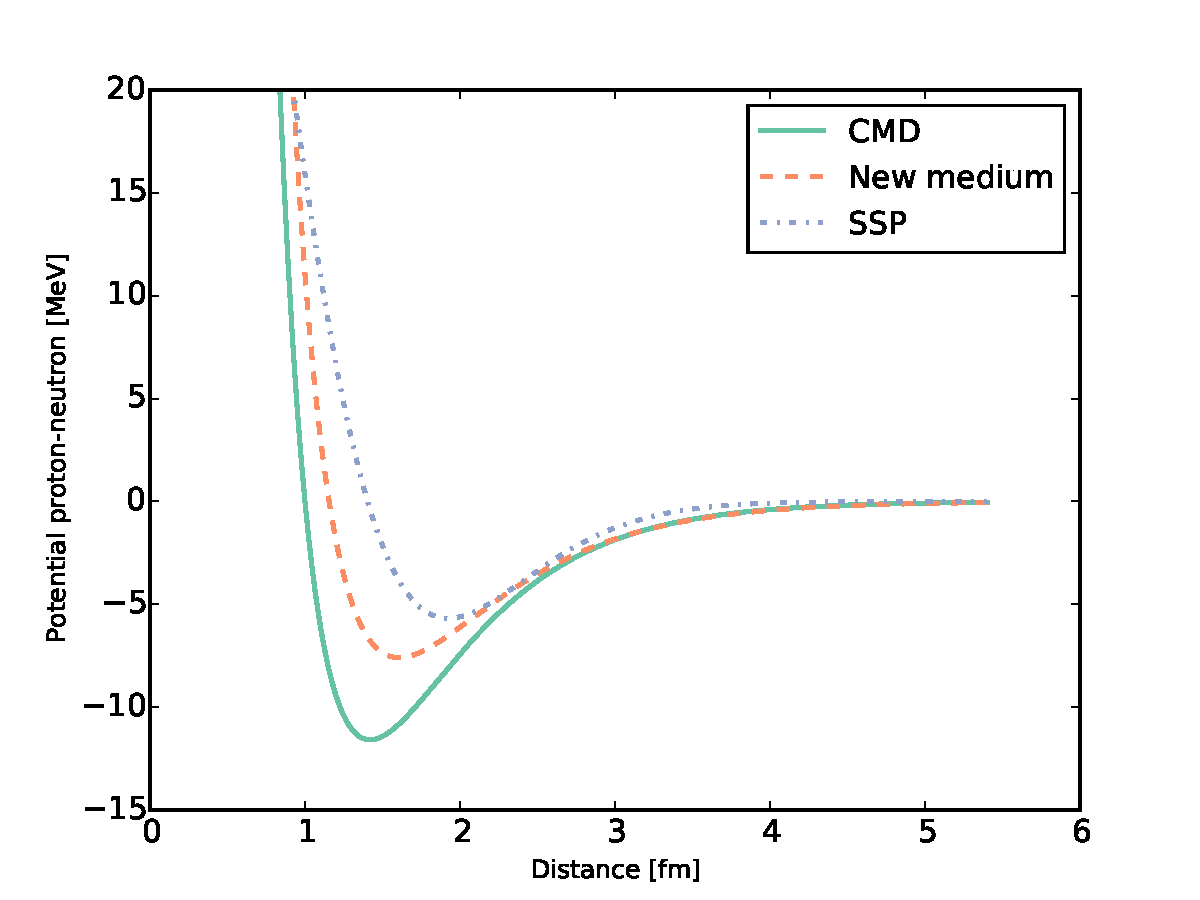
\includegraphics[width=0.7\columnwidth]{introduccion/vnp}
  \caption{Potencial de interacción entre protón y neutrón para distintas parametrizaciones de CMD.}
\label{fig:vnp}
\end{figure}

Para simular un medio infinito, utilizamos este potencial bajo condiciones periódicas de contorno en cajas cúbicas, con distintos valores de fracción de protones, densidades y temperaturas.
En trabajos anteriores~\cite{gimenez_molinelli_finite_2015} estudiamos también el comportamiento de materia nuclear en cajas no-cúbicas.
Para realizar las simulaciones, usamos LAMMPS~\cite{plimpton_fast_1995} con su paquete de GPU~\cite{brown_implementing_2012}.

\subsubsection{Núcleos}
A pesar de que el estado a $T=0$ de esta materia nuclear clásica a densidades normales es un sólido con estructura cúbica simple, los sistemas nuclears pueden ser obtenidos agregando energía cinética a los nucleones.
Construimos estos núcleos confinando los nucleones en un potencial esférico y luego enfriándolos lentamente desde una temperatura elevada hasta que llegan a un estado de equilibrio ligado.
Luego retiramos el potencial confinante y enfriamos el sistema.
La figura~\ref{fig:int_binding} muestra las energías de ligadura de los estados fundamentales de los núcleos experimentales y con distintas parametrizaciones de CMD; ver~\cite{alcain_dynamics_2017} para más detalles.

\begin{figure}[h]
  \centering
  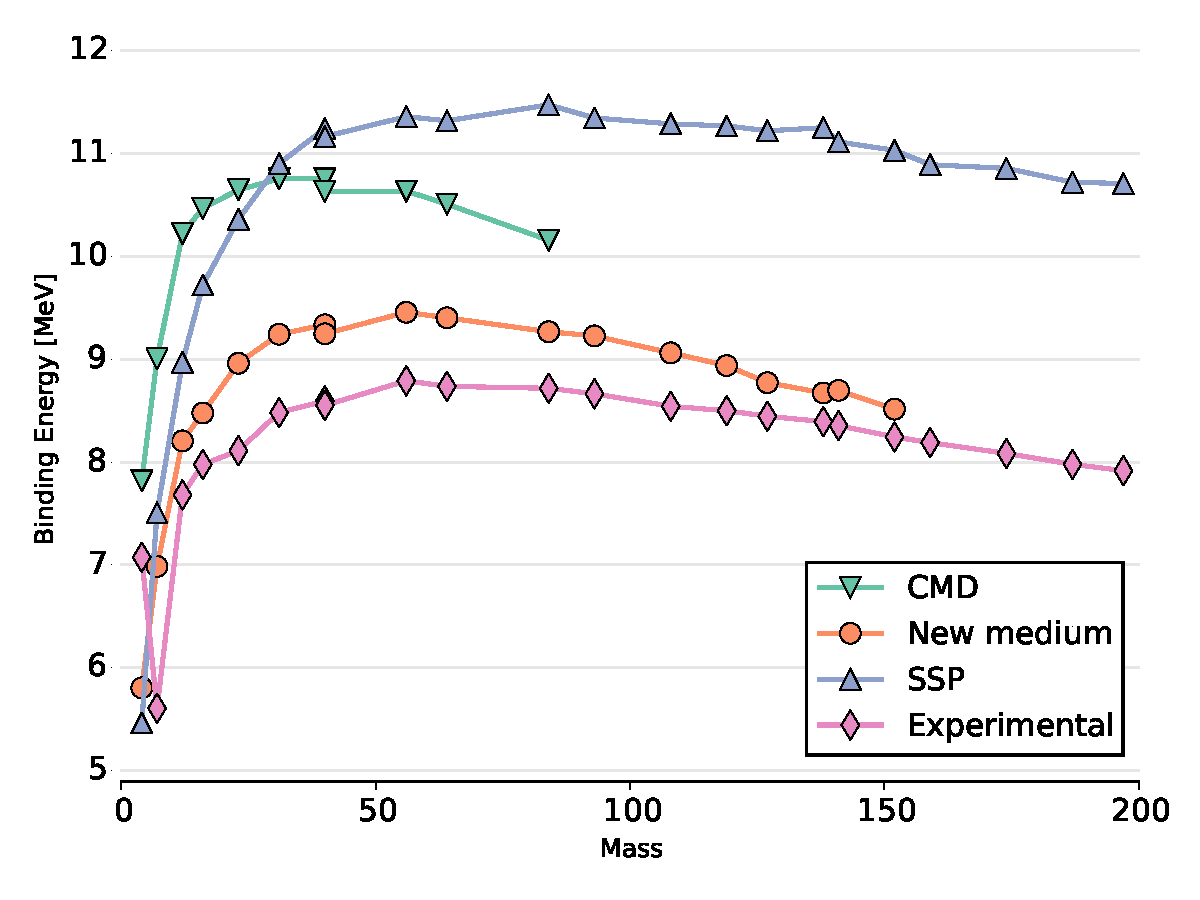
\includegraphics[width=0.7\columnwidth]{introduccion/binding}
  \caption{Energías de ligadura de núcleos obtenidas con CMD, extraída de Ref.~\cite{alcain_dynamics_2017}.}
\label{fig:int_binding}
\end{figure}

\subsubsection{Colisiones Nucleares}
Con respecto a las colisiones, estos potenciales reproducen las secciones eficaces de nucleon-nucleon para energías bajas e intermedias~\cite{lenk_accuracy_1990}, y fue utilizado extensivamente en el estudio de colisiones de iones pesados (ver Ref.~\cite{chernomoretz_quasiclassical_2002, barranon_time_2007}).
Para dichas reacciones, dos núcleos son impulsados uno contra el otro a una energía específica.
Entre colisión y colisión, el proyectil y el objetivo son rotados un con respecto al otro aleatoriamente.
La evolución del sistema se sigue utilizando un algoritmo de Verlet en velocidades, que es simpléctico y conserva la energía al 0.01\%.
A cualquier punto en el tiempo la posición y momento de los nucleones es conocida y puede ser transformada en información de fragmentos y partículas libres a través de distintas técnicas de reconocimiento de fragmentos~\cite{dorso_early_1993, dorso_when_1995, strachan_time_1997}.

Este método implica masas, momentos, energías de excitación y decaimientos secundarios comparables al experimental~\cite{belkacem_searching_1996,chernomoretz_quasiclassical_2002}.
La figura~\ref{fig:distribution}, por ejemplo, muestra las distribuciones de la velocidad paralela simuladas y experimentales obtenidas de la colisión de $\text{Ni+C}$ realizadas en el \emph{Coupled Tandem and Super-Conducting Cyclotron accelerators} de AECL en Chalk River~\cite{chernomoretz_quasiclassical_2002}.

\begin{figure}[h]
  \begin{subfigure}[h!]{0.48\columnwidth}
    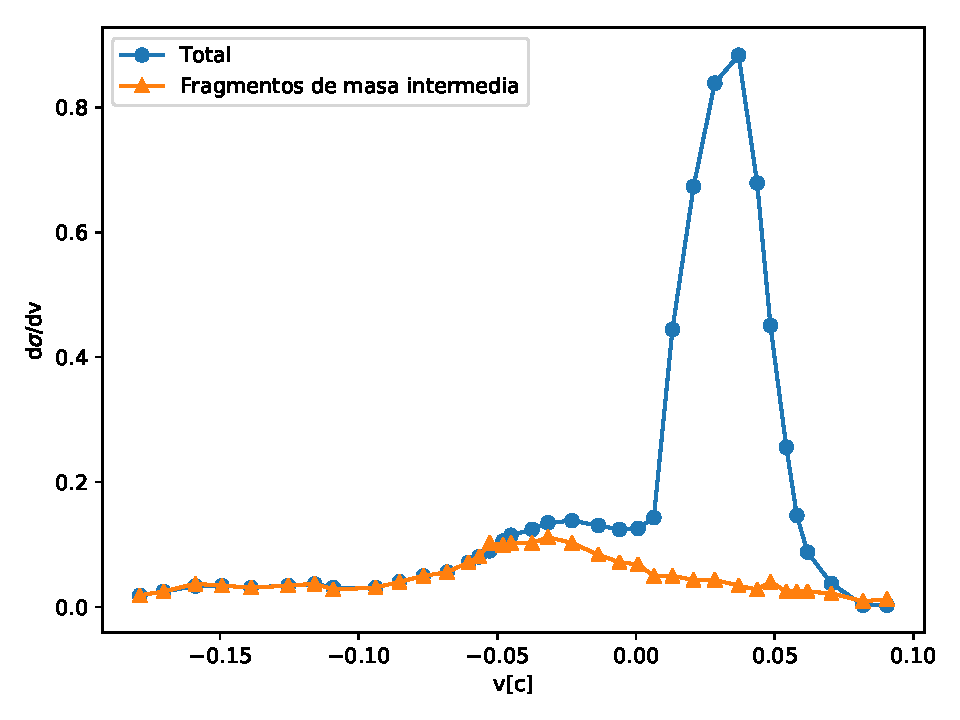
\includegraphics[width=\columnwidth]{introduccion/cherno_experiment}
    \caption{Resultados experimentales.}
    \label{sfig:exp}
  \end{subfigure}
  \begin{subfigure}[h!]{0.48\columnwidth}
    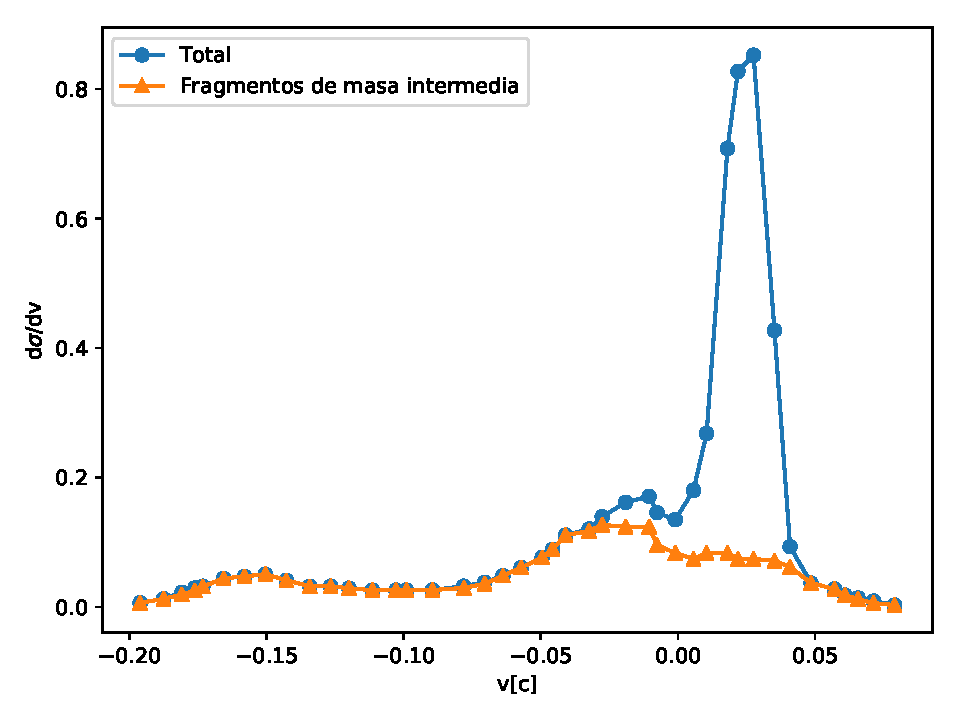
\includegraphics[width=\columnwidth]{introduccion/cherno_simulation}
    \caption{Resultados de la simulación.}
    \label{sfig:sim}
  \end{subfigure}
  \centering
  \caption{Distribuciones de velocidad paralela~\ref{sfig:exp} experimental y~\ref{sfig:sim} simulada para colisiones de ${}^{58}\text{Ni+C}$.}
  \label{fig:distribution}
\end{figure}


\subsubsection{Propiedades termostáticas de la materia nuclear}
Para estudiar las propiedades térmicas de la materia materia nuclear, calculamos la energía para distintos valores de temperatura.
Estos valores de energía por partícula $\epsilon(\rho,T)$ pueden ser utilizados para construir ajustes analíticos, en el espíritu de los de Bertsch, Siemens y Kapusta~\cite{bertsch_nuclear_1983, kapusta_deuteron_1984,
  lopez_nuclear_1984}; estos ajustes, a su vez, pueden ser utilizados para encontrar otras variables termodinámicas y mecánicas, como por ejemplo la presión.

La figura~\ref{fig:energy_nm} muestra los resultados de este método aplicados por Giménez-Molinelli \emph{et al.}~\cite{gimenez_molinelli_simulations_2014} para materia nuclear infinita, simulada en celdas finitas con condiciones periódicas de contorno.
Podemos observar que el cálculo de CMD a bajas temperaturas (\mydiamond{color4}{white}) no coincide con la solución homogénea impuesta para distintas simetrías de los cristales (\mycircle{black}{color1}, \mytriangle{black}{color2}, \mysquare{black}{color3}).
Esto muestra la emergencia de pseudo pastas en materia nuclear.

Para sistemas finitos, la figura~\ref{fig:caloric} muestra el uso de CMD para estudiar las propiedades térmicas, como la curva calórica, para un sistema de 80 nucleones equilibrado a cuatro densidades diferentes; ver Ref.~\cite{dorso_isoscaling_2011} para detalles completos.

\begin{figure}[h]
  \centering
  \begin{subfigure}[h!]{0.48\columnwidth}
    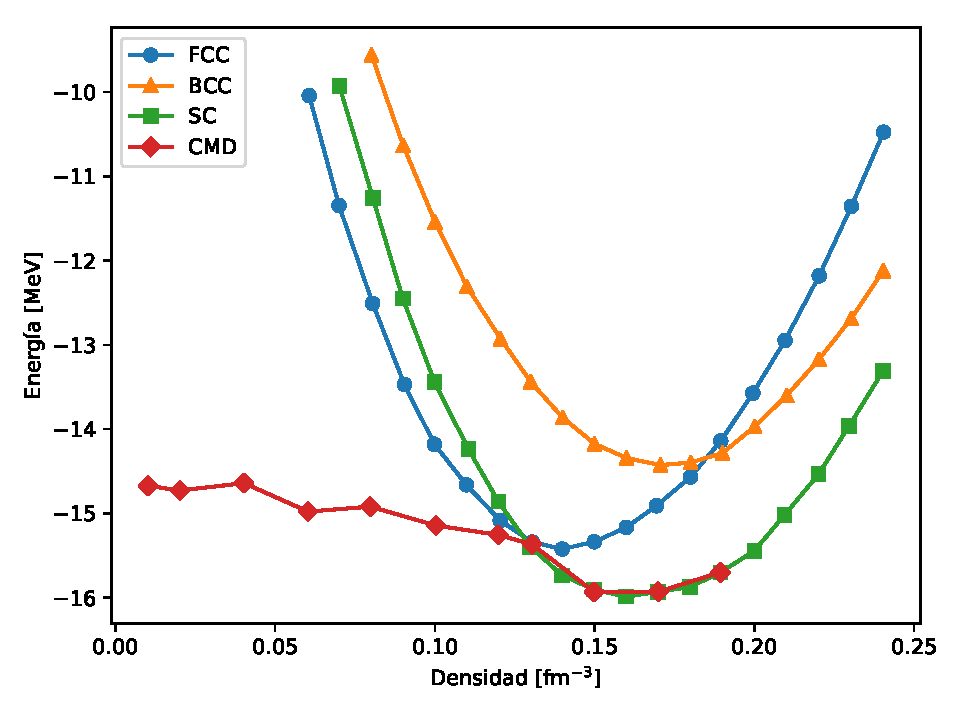
\includegraphics[width=\columnwidth]{introduccion/energy_nm}
  \caption{Energía de la materia nuclear por partícula calculada con CMD y para distintos sistemas homogéneos.}
  \label{fig:energy_nm}
  \end{subfigure}
  \begin{subfigure}[h!]{0.48\columnwidth}
  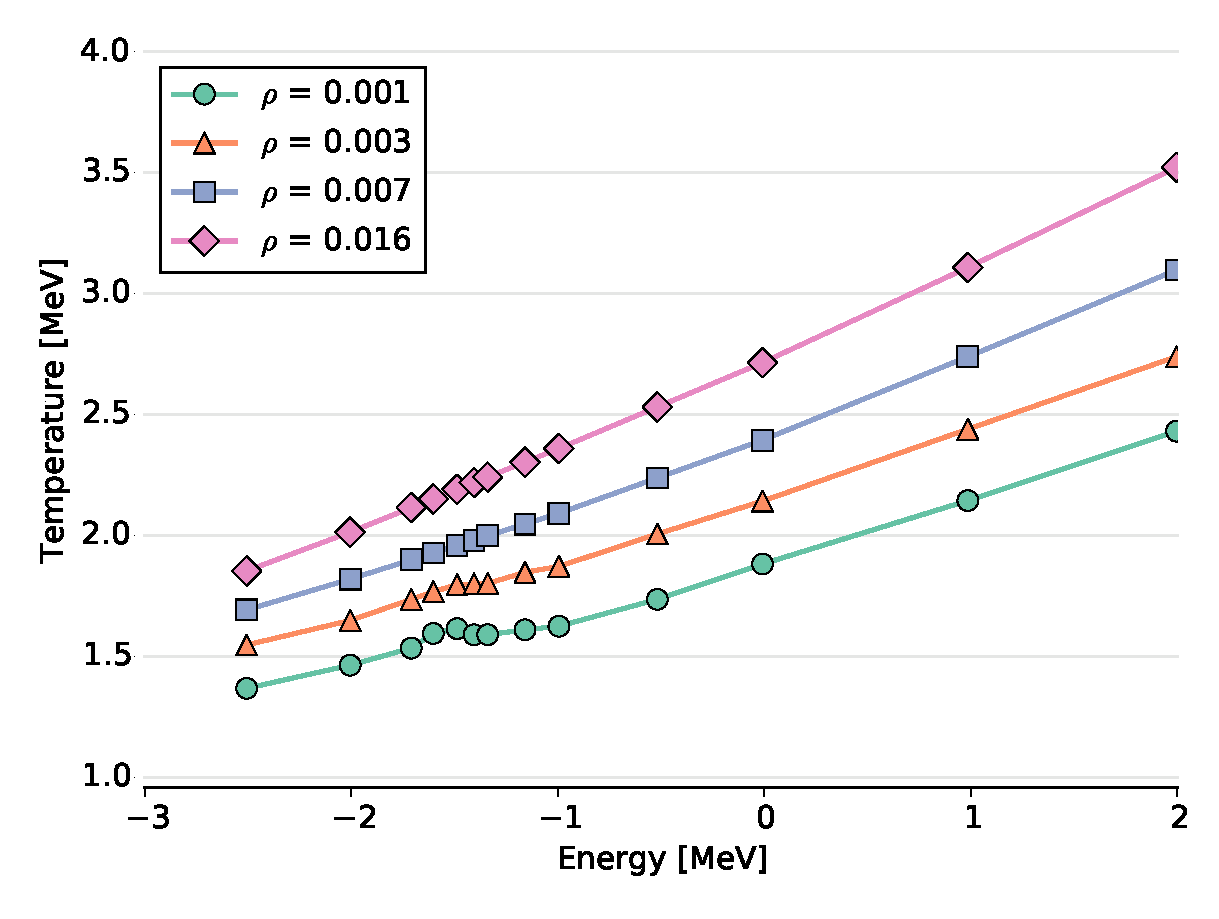
\includegraphics[width=\columnwidth]{introduccion/caloric}
  \caption{Curva calórica de un sistema equilibrado a cuatro densidades diferentes, calculado con CMD.}
  \label{fig:caloric}
  \end{subfigure}
  \caption{Resultados termostáticos para CMD para materia nuclear infinita y para sistemas finitos}
\end{figure}


\subsection{Interacción de Coulomb en el Modelo}\label{sc:coulomb}

Ya que un gas de electrones neutralizante rodea a los nucleones en la corteza de las estrellas de neutrones, las fuerzas de Coulomb entre los protones son apantalladas.
El modelo que utilizamos para este efecto de apantallamiento es la aproximación de Thomas-Fermi, utilizada en varios modelos nucleares~\cite{maruyama_quantum_1998, dorso_topological_2012, horowitz_neutrino-pasta_2004}.
De acuerdo a esta aproximación, los protones interactúan a través de un potencial tipo Yukawa, con una longitud de apantallamiento $\lambda$:
\begin{equation*}
 V_{TF}(r) = q^2\frac{e^{-r/\lambda}}{r}.
\end{equation*}

Estimaciones teóricas para la longitud de apantallamiento $\lambda$ son $\lambda\sim100\,\text{fm}$~\cite{fetter_quantum_2003}, pero escogimos como valor $\lambda=20\,\text{fm}$.
Justificamos esta elección en el capítulo~\ref{ch:coulomb}, donde mostramos que este valor es suficiente para reproducir adecuadamente la longitud de las fluctuaciones de densidad para este modelo, mientras que valores mayores para la longitud de apantallamiento conllevarían a una dificultad computacional.

\section{Estrellas de Neutrones a bajas densidades y temperaturas}\label{sc:nsm_lowd}

Considerar el sistema con una interacción de Coulomb da pie a un fenómeno interesante.
A densidades menores que la de saturación, el sistema exhibe una estructura inhomogénea conocida como pasta nuclear, caracterizada por la emergencia de múltiples estructura por celda de simulación.
Esta pasta nuclear puede ser caracterizada como la original propuesta por Williams y Koonin (ver sección~\ref{sc:intro}): \emph{gnocchi}, \emph{spaghetti}, \emph{lasagna} y túneles.
Como ejemplo, en la figura~\ref{fig:pasta} mostramos las configuraciones de algunas de estas pastas.


\begin{figure}[h]
  \begin{subfigure}[h!]{0.48\columnwidth}
    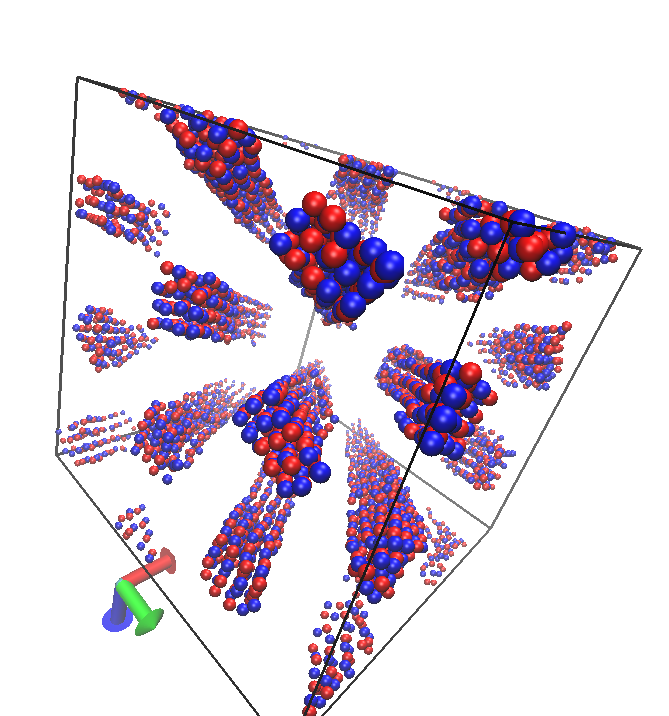
\includegraphics[width=\columnwidth]{introduccion/spaghetti}
    \caption{$\rho = 0.03\,\text{fm}^{-3}$}
    \label{sfig:spaghetti}
  \end{subfigure}
  \begin{subfigure}[h!]{0.48\columnwidth}
    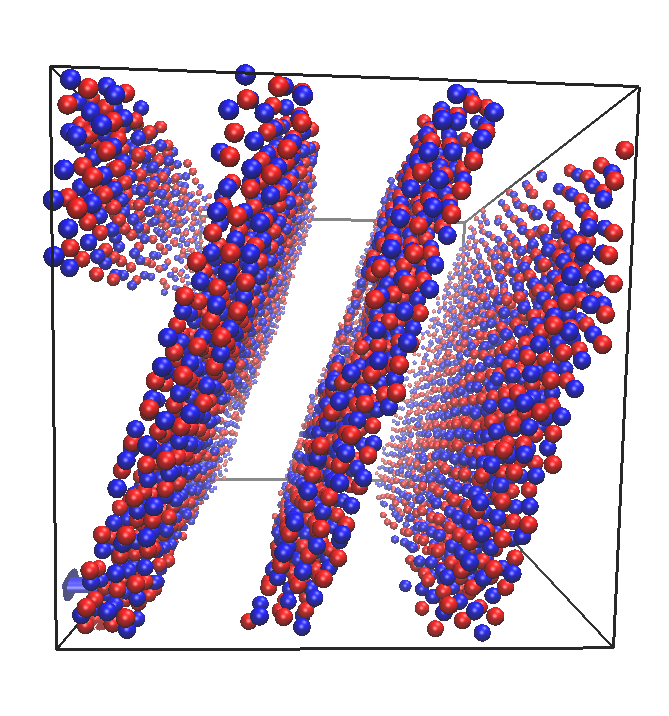
\includegraphics[width=\columnwidth]{introduccion/lasagna}
    \caption{$\rho = 0.05\,\text{fm}^{-3}$}
    \label{sfig:lasagna}
  \end{subfigure}
  \begin{subfigure}[h!]{0.48\columnwidth}
    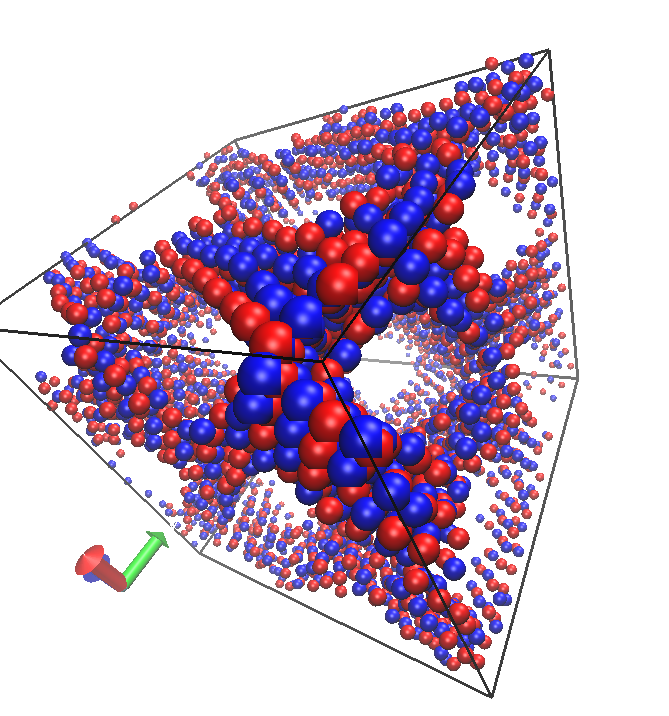
\includegraphics[width=\columnwidth]{introduccion/tunnels}
    \caption{$\rho = 0.08\,\text{fm}^{-3}$}
    \label{sfig:tunnels}
  \end{subfigure}
  \centering
  \caption{\ref{sfig:spaghetti} Spaghetti,~\ref{sfig:lasagna} lasagna y~\ref{sfig:tunnels} túneles obtenidos con CMD, para el caso simétrico en isospín $x=0.5$ y baja temperatura $T=0.5\,\text{MeV}$, extraído de Ref.~\cite{alcain_effect_2014}}
  \label{fig:pasta}
\end{figure}

\section{Choque de Estrellas de Neutrones}

El 17 de agosto de 2017, LIGO observó ondas gravitacionales surgidas de la colisión de dos estrellas de neutrones~\cite{ligo_scientific_collaboration_and_virgo_collaboration_gw170817:_2017}.
Son consideradas como fuentes posibles de nucleosíntesis generadas por el proceso de captura rápida de neutrones, conocido como \emph{r-process}.
Su aporte a la abundancia terrestre de núcleos terrestres aún está en discusión, pero se especula que es responsable de más de la mitad de los elementos con masa mayor a la del hierro y la única fuente de elementos más pesados que el plomo.
La simulación con detalle microscópico de la colisión de Estrellas de Neutrones imposible en la práctica, ya que implicaría la simulación de $10^{55}$ partículas sólo en la corteza y la interacción de $10^{110}$ pares de partículas, por lo que usualmente estos estudios se realizan con un enfoque hidrodinámico más característico de las técnicas de campo medio.
De este modo se intenta emular el comportamiento microscópico en la simulación detallada de la colisión.

La otra alternativa es emular la colisión en el ambiente microscópico.
Para lograrlo sometemos a un sistema de protones y neutrones a una expansión homogénea, conocida como pequeño \emph{big bang}~\cite{dorso_onset_1996}.



%  LocalWords:  MeV fm neutron lasagna spaghetti gnocchi Ref Coupled
%  LocalWords:  Tandem and Super Conducting Cyclotron
